\chapter{RESULTS}
\thispagestyle{plain}

\label{Results}

In this chapter, I discuss experiments that test the  accuracy and computational efficiency of \fw.
These experiments also serve as examples of \fw being applied to a variety of ABMs.
In the next section, the different evaluation criteria are outlined.
Each of these metrics will be applied to a number of domains using a number of different techniques for the forward mapping.
The four domains used for the sake of experimentation were outlined in Chapter \ref{Domains}.
Each of these domains have unique properties that provide unique challenges to show the versatility of \fw.
The different regression methods for the forward mapping are outlined in Section \ref{sec:fmalgo}.
Finally, in Section \ref{sec:exps}, the statistical results are discussed.

\section{Evaluation}

Evaluating \fw is important because it shows that the framework is a practical and useful tool for studying ABMs.
Evaluation is split into two processes: evaluating the forward mapping solution and evaluating the reverse mapping solution.
Accuracy of these mappings in modeling the behavior space of the target ABM is paramount in importance.
If the forward and reverse mappings are not accurate, there would be no reason to use this framework for investigating behaviors of ABMs.
Computation time is also an important factor in evaluating \fw.
Interactions with the user need to be quick in order to make using \fw more convenient than manually inspecting the target ABM.
The response time of when a user interacts with \fw is the \textit{online} time and is far more important than the \textit{offline} time, the one-time computation requirement to learn the forward or reverse mapping.


 \subsection{Forward Mapping}

  \subsubsection{Accuracy}
Accuracy is the measurement of how closely the forward mapping represents the true behavior space of a target ABM.
To measure this, the difference (error) $\varepsilon$ between the predictions for a system level property $\hat y$ that the forward mapping produces and the actual value $y$ for a sampled point: $\varepsilon = |\hat y - y|$.
This measurement is performed many times for a single domain to produce the median error and the the upper and lower quartiles of the errors.

The errors are gathered by performing cross validation.
Two subsets of data points are randomly pulled from the master set of samples to create a training set and a validation set.
The forward mapping is built by using the training set, and then checked with the validation set.

The error is calculated for varying size data sets to show the relationship between error and data set size.

  \subsubsection{Offline Computation Time}

Offline computation time is the average amount of system time the forward mapping uses to train a model.
This is measured as the amount of time the pre-processing takes, given a training set.
The size of the training set is varied to determine how forward mapping training time is correlated to training set size.
Each forward mapping method is compared to the others.

  \subsubsection{Online Computation Time}

Online computation time is the average amount of time \fw takes to return the results of a user-submitted query.
This is measured by performing a large number of queries and calculating the average run time.
The size of the training set can affect the amount of time a query will take with some algorithms.
In these cases, the size of the training set is varied to determine how query time correlates to training set size.

 \subsection{Reverse Mapping}

  \subsubsection{Accuracy vs. Forward Mapping}
Accuracy of the reverse mapping is measured in two ways.
The first is how accurately the reverse mapping models the forward mapping.
Recall that \fw solves the reverse mapping by building an invertible approximation of the forward mapping.
This metric determines if this approach is doing what is expected to do.
The effect that granularity has on this accuracy is also measured by learning the same mapping with increasingly higher granularity.

\begin{figure}[ht]
\centering
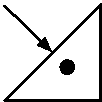
\includegraphics[scale=1]{images/mosterror.pdf}
\caption{The most erroneous spot in a right-angled simplex.}
\label{fig:mosterror}
\end{figure}

The error is presented as an ``average worst-case scenario".
The area of the reverse mapping space that is be the most erroneous is typically be the one furthest from the knots (corners of the simplex).
An illustration of this point is presented in Figure \ref{fig:mosterror}.
The point is halfway between all corners, except for the corner at the right angle.
This point is the most erroneous if the forward mapping is monotonically changing from one side of the simplex to the other (i.e., there are no local maxima or minima within the space).
Note that the reverse mapping will be identical to the forward mapping at the knots, since the forward mapping was used to infer their values.

Calculating the approximate upper bound on error, within a simplex, involves interpolating the system-level property value at the most erroneous point.
This is done by average the system-level property values of all corners not at the right angle.
Also, the location of the most erroneous point is queried for prediction through the forward mapping.
The difference between the interpolated value on the simplex and the actual predicted value using the forward mapping constitutes the error.
This metric is applied for every simplex and then averaged.
Thus, the metric measures the average error over all the worst-case scenarios for each simplex.
Also, the distribution of these errors is recorded to convey how consistent the reverse mapping is.


  \subsubsection{Accuracy vs. Agent-Based Model Run}

The main goal of the reverse mapping is to be able to suggest configurations that would generate a specified behavior.
This approach is different from the previous metric because it measures the difference between the reverse mapping and the true behavior space.

\begin{figure}[ht]
\centering
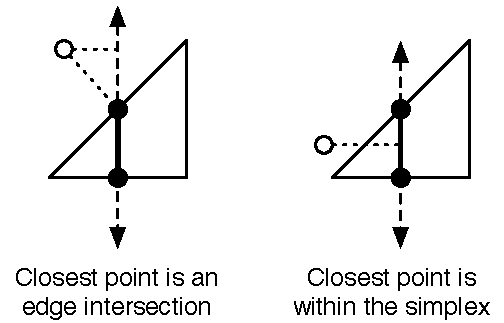
\includegraphics[scale=1]{images/closest.pdf}
\caption{Two cases for the closest point to a simplex intersection.}
\label{fig:closest}
\end{figure}

Error is measured by generating a random configuration point and sampling it from the agent-based model.
Then, the system-level property that was measured is passed to \fw to generate a reverse-mapping solution.
The error is the distance from the original configuration and the reverse-mapping solution space.
This value is calculated by adhering to the following procedure, per simplex:
\begin{enumerate}
  \item Determine the distance from the original point to the intersecting hyperplane.
  \item If the shortest line from the hyperplane to the point intersects the hyperplane \textit{within} the simplex, then the distance from the hyperplane is the distance from the intersection to the point.
  \item Otherwise, the closest point is one of the edge intersections.
\end{enumerate}
The two different cases (closest to an edge (left) and closest to the hyperplane (right)) are illustrated in Figure \ref{fig:closest}.
The minimum of all of these closest simplex points is taken as the distance from the actual system-level property value to the piecewise curve generated by the reverse mapping.


Several random configurations are sampled in this way.
The average and standard deviation of these errors are calculated to convey the accuracy of the reverse mapping, as well as the consistency of the reverse mapping.

  \subsubsection{Offline and Online Computation Time}
Offline computation time and online computation time is measured the same way for the reverse mapping as the forward mapping.
The amount of time \fw takes to prepare the reverse mapping is the offline computation time, and the amount of time required to produce a reverse mapping solution is the online computation time.



\section{Forward Mapping Methods}\label{sec:fmalgo}

For the experiments in this chapter, the three algorithms described in Chapter \ref{Background} are used for the forward mapping. In the following outline, I indicate specific configuration parameters or implementation details of importance.
\begin{itemize}
 \item k-nearest neighbor (KNN)
  \begin{itemize}
   \item Custom implementation with Python.
   \item 10-fold validation is used to determine the best $k$ out of a set of possible $k$ values.
  \end{itemize}

 \item robust locally weighted regression and smoothing scatterplots (LOESS)
  \begin{itemize}
   \item Custom implementation with Python.
   \item A good window is selected by myself for each domain. Changing this configuration parameter per sample size does not affect accuracy, as it does with kNN.
   \item Performs one smoothing operation. I found that increasing the number of smoothing operations past one provided limited improvement in accuracy and occasionally worsening accuracy. Finding an optimal smoothing with cross validation, per training set, would be computationally expensive.
  \end{itemize}

 \item nonlinear regression (NLR)
   \begin{itemize}
      \item Implemented in Python and uses the SciPy\footnote{SciPy is a freely available Python module that has a number of useful computational tools. The SciPy website is: http://www.scipy.org/} package to optimize the parametric model with least-squares.
   \end{itemize}

\end{itemize}


\section{Experiments}\label{sec:exps}

First, I will discuss results from the Fires domain together, which provides an extended example that explains the methodology and results for each of the seven experiments.
The rest of the experiments  for the other domains are grouped together by experiment, so that the effectiveness of the different components of \fw are evaluated independently.

 \subsection{Fires Domain Experiments}

The NetLogo Fires domain is an excellent example for showing how \fw works, as the domain is relatively simple and easy to visualize.
Plots of the behavior space for this domain are shown in Figure \ref{fig:rii}.


%training sizes of 20-200 (step 20)
% fm was trained 20 times per training set size
% 15 different validation sets were used on 15 different fm from different validation sets
% validation set size 2500
% granularities 25-300 (step 25)
% rm was retrained 15 times and validated with the 2500 points
% rm uses kNN with the highest data set size (200)


\subsubsection{Forward Mapping Training Time}


\begin{figure}[ht]
\centering
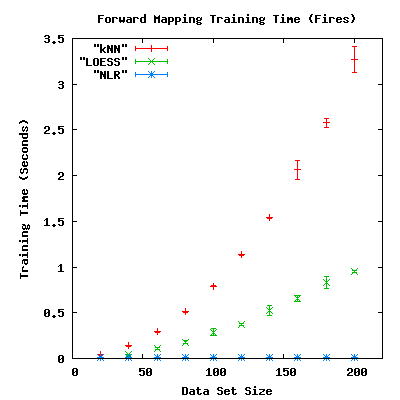
\includegraphics[scale=.5]{images/results_fires/fmtraining.png}
\caption{The average length of time required by the forward mapping for the Fires domain to train.
The error bars show the 95\% confidence interval for the mean.}
\label{fig:firefmtraining}
\end{figure}

Different training data set sizes, ranging from 20 to 200 (with a step of 20), were used to measure the amount of computation time the forward mapping requires to train a model.
Each of the three regressions were retrained twenty times per training data set size.
The results are plotted in Figure \ref{fig:firefmtraining}.
This plot shows that kNN grows faster than the other two approaches with increasing data set sizes.
This is because the 10-fold validation for picking $k$ requires a significant amount of time.
Meanwhile, LOESS grows at a linear rate.
The training time for NLR is insignificant in comparison to the other approaches.
Least-squares optimization is a mature subject area, and SciPy uses some of the most advanced methods to make the optimization quick.

Even the slowest of these regressions, kNN with 200 training instances, runs in only 3.25 seconds, which is acceptable for a one-time process.


The error bars show that there is little variability in training time, meaning that the approaches are consistent in the amount of time they take.


\subsubsection{Forward Mapping Accuracy}

\begin{figure}[ht]
\centering
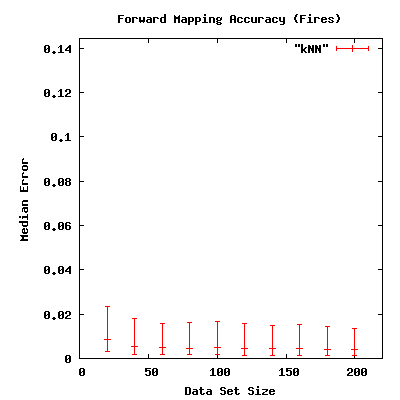
\includegraphics[scale=.3333333]{images/results_fires/fmacc-kNN.png}
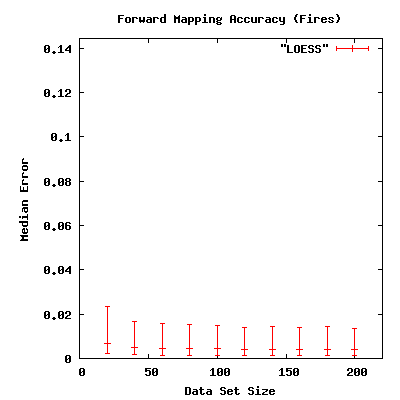
\includegraphics[scale=.3333333]{images/results_fires/fmacc-LOESS.png}
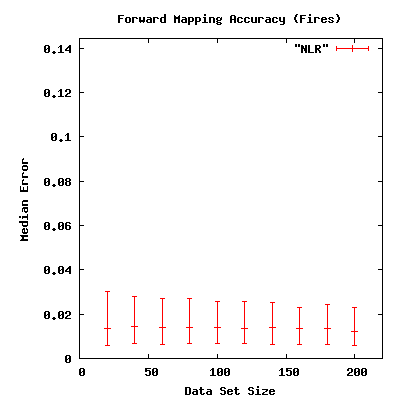
\includegraphics[scale=.3333333]{images/results_fires/fmacc-NLR.png}
\caption{The median error (in ratio of trees burned down) for three different forward mapping regression methods.
The error bars show the upper and lower quartile of the errors, over all trials.}
\label{fig:fmacc}
\end{figure}

Different training data set sizes, ranging from 20 to 200 (with a step of 20), were used to train a model.
Fifteen different training data sets were produced per data set size.
For each of these trained models, 2500 points from a validation set were used to evaluate the accuracy of the forward mapping, in respect to values sampled directly from ABMs.
The configuration of each validation instance was passed into the forward mapping to retrieve a predicted value.
This predicted value was then compared to the sampled value from the validation instance to produce an error value.

The accuracy of the forward mapping is very high, for all three approaches: all three approaches predict the amount of trees burned down within an accuracy of 1\%.
The median error, along with the upper quartile and lower quartile are plotted in Figure \ref{fig:fmacc}.

This is impressive considering to the amount of variability from sample to sample of the Fires domain.
Both KNN and LOESS perform better with more data points, however with a sample size greather than 80, the accuracy does not appear affected very much.
Overall, KNN had a lower median error than LOESS, but not by a statistically significant amount.
NLR performed worse than the other two approaches and experienced more variance in its errors.
Interestingly, the accuracy of NLR only slightly improved from a data sample size of 20 to a data sample size of 200.
Since NLR is a parametric approach, the optimal model for a small number of points will be very similar to the optimal model for a large number of points from the same distribution.
Meanwhile, locally weighted nonparametric approaches have the ability to fit sections of the behavior space more closely as more points are provided.
This trade off is demonstrated in the accuracy results.


\subsubsection{Forward Mapping Query Time}
\begin{figure}[ht]
\centering
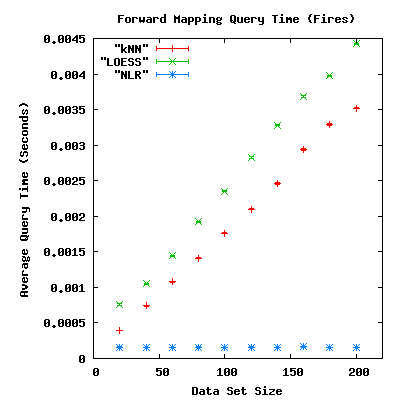
\includegraphics[scale=.5]{images/results_fires/fmquery.png}
\caption{The average number of seconds required to query the Fires forward mapping.
The error bars show the 95\% confidence interval for the mean.}
\label{fig:firefmquery}
\end{figure}

Measurements of the query time were performed at the same time as the accuracy measurements.
The elapsed time was measured for every prediction call to the forward mappings.

Queries to the forward mappings for the three approaches are fast, as illustrated in Figure \ref{fig:firefmquery}.
The longest time for a query to execute was .0045 seconds for LOESS using a data set of size 200.
This amount of time is instantaneous to a human user and thus satisfies the requirement that the forward mapping is fast for the user.
As expected, data set size has no effect on the computation time of NLR because the model equation is always the same number of parameters.
Also, as expected, LOESS and kNN query time grows linearly with the size of the data set.
For every new point added, an additional point must be checked to see if it is local to the passed in configuration, or not.


\subsubsection{Reverse Mapping Training Time}

\begin{figure}[ht]
\centering
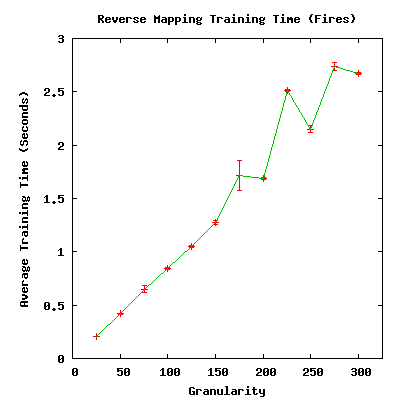
\includegraphics[scale=.5]{images/results_fires/rmtraining.png}
\caption{The average number of seconds required to train the Fires reverse mapping.
The error bars show the 95\% confidence interval for the mean.}
\label{fig:rmtraining}
\end{figure}

The most accurate forward mapping trained in the previous forward mapping experiments was used for the reverse mapping experiments.
In this case, I used kNN with a training set of 200.
Training time was measured for reverse mappings training on granularities of 25 to 300 (step 25).
A granularity of $N$ means the configuration space was split into $N$ simplexes, per dimension.
The test was repeated fifteen times per granularity.

The training time increased linearly with an increase in granularity.
With a granularity of three hundred, the training time was under three seconds.
With a granularity of twenty-five, the training time was just under a quarter of a second.


\subsubsection{Reverse Mapping Accuracy}

\begin{figure}[ht]
\centering
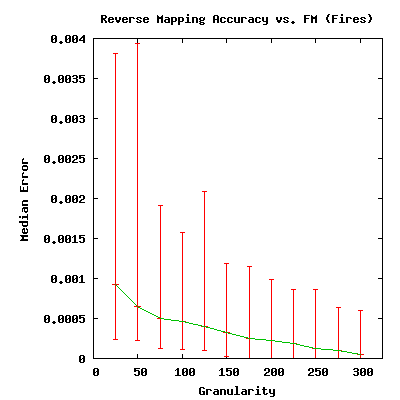
\includegraphics[scale=.5]{images/results_fires/rmaccfm.png}
\caption{The median distance from the suggested tree density (0-100) to the one predicted by the forward mapping.
The error bars show the upper and lower quartile of errors measured.}
\label{fig:rmaccfm}
\end{figure}

The reverse mapping accuracy is measured in two ways.
First, I measured the median error of the reverse mapping in respect to the predicted values of the forward mapping.
This metric demonstrates the accuracy of fifteen different reverse mappings per granularity, as an approximation of the forward mapping.
This metric is measured by taking each simplex in the reverse mapping and selecting the furthest point from the corners.
Each of these points are then passed to the forward mapping to provide a prediction, which is then compared to the interpolated value within the simplex.
The difference between these two denote the error of the values within the simplex, in respect to the forward mapping it is approximating. 

Figure \ref{fig:rmaccfm} shows the effect of granularity on median error.
The error steadily decreases with higher granularity, eventually approaching 100\% for about half of the queries.
Also, the error is extremely low in all cases, never exceeding half a percent of trees burned down.
The reverse mappings trained with high granularities were often accurate within a tenth of a percent of trees burned down.

\begin{figure}[ht]
\centering
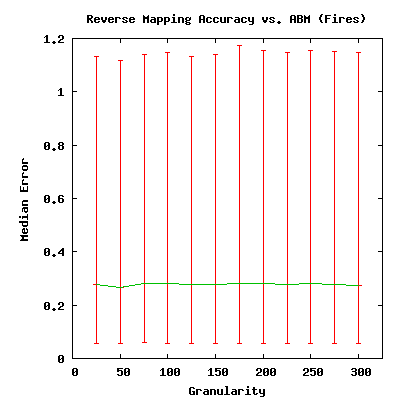
\includegraphics[scale=.5]{images/results_fires/rmaccabm.png}
\caption{The median distance from the suggested tree density (0-100) to the actual tree density.
The error bars show the upper and lower quartile of errors measured.}
\label{fig:rmaccabm}
\end{figure}
The second way the accuracy of the reverse mapping is measured is how distant the piecewise configuration curve returned by the reverse mapping is from the actual configuration.
Recall that the reverse mapping returns a set of intersections (however, in the case of Fires typically only one, since the mapping is one-to-one).
This metric intends to measure the distance from a configuration suggested by the reverse mapping, and the actual configuration from the validation set.
Each of the 2500 instances from the validation set were used for each of the reverse mappings that were trained.

The results in Figure \ref{fig:rmaccabm} show that the median error remains fairly constant, regardless of granularity.
The reason for this is that the error incurred by the approximation of the forward mapping is insignificant in comparison to the error of kNN.
Since the same kNN forward mapping was used for all granularities, the error incurred by the reverse mapping is not noticeable or statistically significant.


\subsubsection{Reverse Mapping Query Time}

\begin{figure}[ht]
\centering
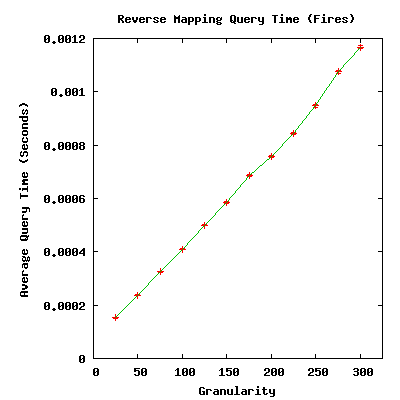
\includegraphics[scale=.5]{images/results_fires/rmquery.png}
\caption{The average number of seconds required to queury the Fires reverse mapping.
The error bars show the 95\% confidence interval for the mean.}
\label{fig:rmquery}
\end{figure}

The reverse mapping query time was measured along with the accuracies of the reverse mapping, in respect to the validation set.

Overall, the average reverse mapping query computation time is almost instantaneous, taking about 0.0012 seconds with a granularity of 300, as seen in Figure \ref{fig:rmquery}.
The average query time increased linearly with the granularity because each additional simplex must be checked for intersections.


 \subsection{Forward Mapping}

  \subsubsection{Accuracy}

The accuracy of the forward mapping was measured in the three remaining domains (Flocking, AIDS and Wolf Sheep Predation).
In all domains, both k-nearest neighbor and LOESS outperformed the baseline of predicting the mean value over all system-level property values.
Also, all experiments demonstrate that, in general, accuracy increases as data set size increases.
However, the decrease in error from increasing data set size is not a linear relationship, as the benefits of larger datasets lessens as the size increases.
In general, kNN performed better than LOESS.
Non-linear regression has been omitted from these experiments for the reason that it is difficult to determine a suitable base-model and initial guess for a multi-dimensional space.

\begin{figure}[ht]
\centering
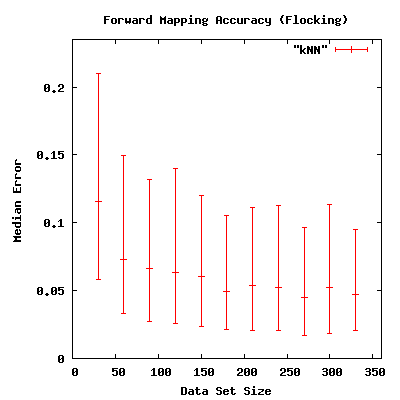
\includegraphics[scale=.4]{images/results_flocking/fmacc-kNN.png}
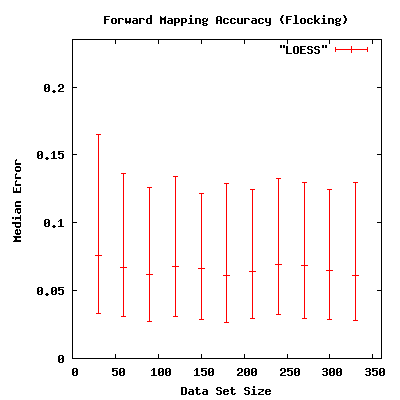
\includegraphics[scale=.4]{images/results_flocking/fmacc-LOESS.png}
\caption{The median error for the standard deviation of heading (on a zero-to-one scale) in the Flocking domain for two different forward mapping regression methods.
The error bars show the upper and lower quartile of the errors, over all trials.}
\label{fig:flockfmacc}
\end{figure}

Both LOESS and kNN were tested for training a forward mapping to predict the standard deviation of heading in the Flocking ABM.
A forward mapping was trained fifteen times for each data set of the same size, each being queried one thousand times.
Plots showing the relationship between data set size and median error are shown in Figure \ref{fig:flockfmacc}. 
KNN outperformed LOESS, but not significantly, eventually approaching a median error of .05 with a training set size of 325.
LOESS approached an error of .06 with the same training set size.
These error values are linearly scaled such that the maximum standard deviation witnessed is exactly 1.0 and the minimum standard deviation witnessed is exactly 0.0.
The baseline is not shown in these graphs because it is not within the $y$-range of the plot: on average, predicting the mean value had an error of .306, over all 4000 data set instances.


\begin{figure}[ht]
\centering
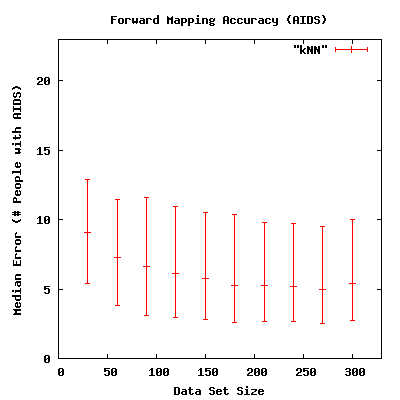
\includegraphics[scale=.5]{images/results_aids/aids-fmacc.png}
\caption{The median error showing the difference in people  (out of 350) between the original curve and the curve predicted by the forward mapping, on average, over all time steps.
The error bars show the upper and lower quartile of the errors, over all trials.}
\label{fig:aidsfmacc}
\end{figure}

Four forward mappings were trained to predict four parameters of a generalized logistic function that models the number of people with HIV, in respect to time.
The model used was:
\[ \mathrm{y} = p_0 + \displaystyle \frac{p_1 - p_0}{1 + e ^ {-p_2  (\mathrm{t} - p_3) } }, \]
where $\mathbf p$ is the vector of parameters $p_0, p_1, p_2,$ and $p_3$ and $t$ is the time step.
As the data set size increases from 25 to 300, the median error drops from nine people to just over five, as seen in Figure \ref{fig:aidsfmacc}.
This error is measured by taking the average difference between the predicted curve and the actual curve from the validation set.
To calculate this, the value for each time step, for both functions is calculated.
The deviations are averaged, which yields the median error plotted in Figure \ref{fig:aidsfmacc}.

Note that the AIDS domain technically does not adhere to one of the major assumptions used in \fw: in order to split the forward-mapping problem into several subproblems, the system-level property values must be independent of one another.
This is not the case since all the parameters are part of the same model function.
However, I found that in this particular case, the forward mapping predicted the values of the HIV population adequately.


\begin{figure}[ht]
\centering
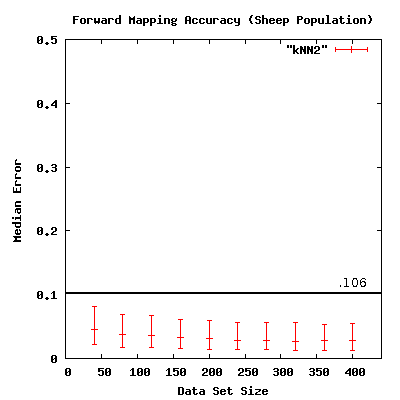
\includegraphics[scale=.4]{images/results_wolfsheep/fm-sheep-pop.png}
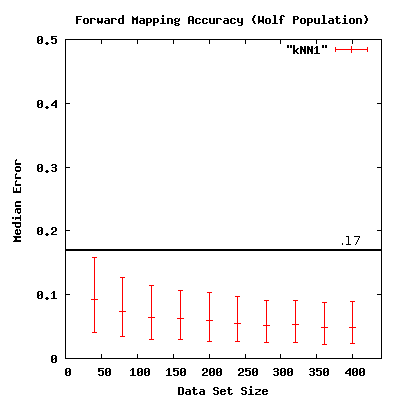
\includegraphics[scale=.4]{images/results_wolfsheep/fm-wolf-pop.png}
\caption{The median error in the average number of sheep (left) and the average number of wolves (right), scaled from zero to one.
The error bars show the upper and lower quartile of the errors, over all trials.
Predicting the mean population value yields an error of .106 and .17 for sheep and wolf populations, respectively.}
\label{fig:wolfsheeppop}
\end{figure}

The next round of experiments tested the effectiveness of the forward mapping approach in predicting four properties of the Wolf Sheep Predation domain: the average sheep population, the average wolf population, the sheep population variance, and wolf extinction.
A forward mapping was trained eight times for each data set of the same size, each being queried two hundred times.
The forward mappings outperformed simply predicting the mean value in all four cases, with sufficient training sets.

The median errors for the wolf population and the sheep population are shown in Figure \ref{fig:wolfsheeppop}.
As the training set size approached 400, the error for the sheep population forward mapping approached 2\% of the range of values in the data set, which is five times more accurate than predicting the mean.
The forward mapping for the wolf population was more difficult to learn, which is evident from the baseline of .17 being significantly higher than the baseline for the sheep population prediction.
The median error for the wolf population forward mapping approaches 4\% of the range of values in the data set, which is 4.25 times more accurate than predicting the mean.

\begin{figure}[ht]
\centering
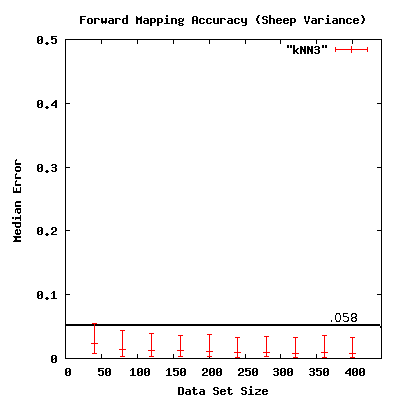
\includegraphics[scale=.5]{images/results_wolfsheep/fm-sheep-var.png}
\caption{The median error of the variance in the number (scaled from zero to one) of sheep.
The error bars show the upper and lower quartile of the errors, over all trials.}
\label{fig:wolfsheepvar}
\end{figure}

Forward mappings were used to predict the variance in sheep populations.
Populations with higher variance fluctuated more than ones with lower variance.
The median error for predicting the variance, based on data set size is shown in Figure \ref{fig:wolfsheepvar}, along with a baseline of .058.
With a training set size of 400, the learned forward mapping outperformed the baseline five-fold.

\begin{figure}[ht]
\centering
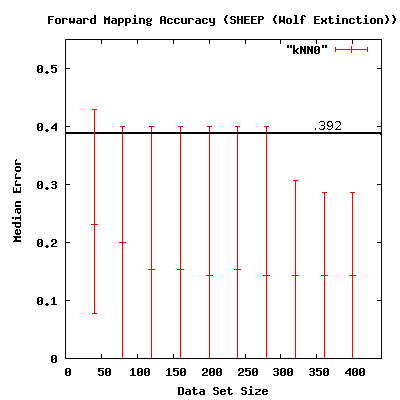
\includegraphics[scale=.5]{images/results_wolfsheep/fm-wolf-extict.png}
\caption{The error in prediction of the wolf population going extinct or not.
The error bars show the upper and lower quartile of the errors, over all trials.}
\label{fig:wolfsheepextinct}
\end{figure}

Next, forward mappings were used to predict whether or not the wolf population would go extinct.
This property is different from the others, since it is a binary property: either the wolves go extinct or they do not.
The forward mapping solution predicts the probability that the wolves go extinct, so the errors shown in Figure \ref{fig:wolfsheepextinct} do not quite have the same meaning as the other plots.
The data in the training set is either labeled as wolves having gone extinct or not.
Therefore, a prediction of .9 would yield an error of .1 if the wolves went extinct, and an error of .9 if they did not.
From the plot in Figure \ref{fig:wolfsheepextinct}, we can see that a forward mapping can be used to predict if the wolves will go extinct correctly the vast majority of the time (at least 75\%).
Also, with a data set size of 400, the forward mapping is more than twice as accurate in comparison to the baseline.

In conclusion, the \fw approach of solving the forward-mapping problem is sufficiently accurate in predicting system-level behavior in these domains.

  \subsubsection{Offline Computation Time}

\begin{figure}[ht]
\centering
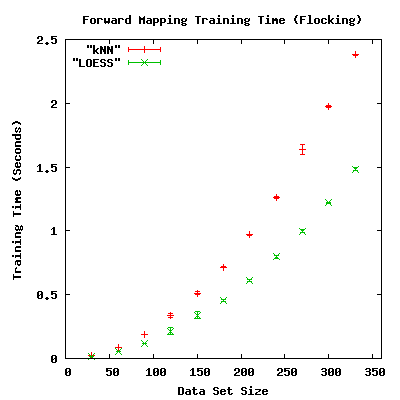
\includegraphics[scale=.4]{images/results_flocking/fmtraining.png}
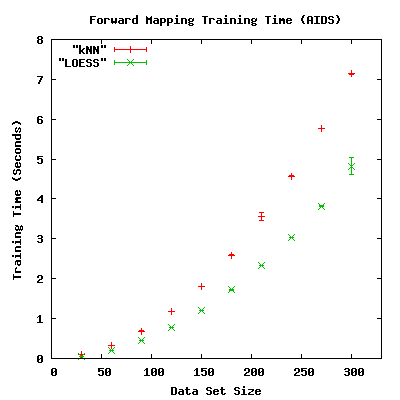
\includegraphics[scale=.4]{images/results_aids/aids-fmtraining.png}
\caption{The average number of seconds required to train the Flocking (left) and AIDS (right) forward mappings.
The error bars show the 95\% confidence interval for the mean.}
\label{fig:fmtraining}
\end{figure}

\begin{figure}[ht]
\centering
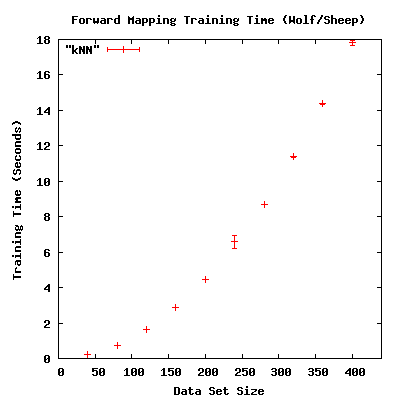
\includegraphics[scale=.5]{images/results_wolfsheep/fm-training.png}
\caption{The average number of seconds required to train the Wolf Sheep Predation forward mapping.
The error bars show the 95\% confidence interval for the mean.}
\label{fig:wolfsheepfmtraining}
\end{figure}

Offline computation time refers to the required amount of time to train a forward mapping.
Recall that kNN determines the best $k$ using 10-fold cross validation and LOESS performs the initialization and smoothing step.
To measure the average training, several forward mappings for all three domains were trained for varying data set sizes.
Figure \ref{fig:fmtraining} shows the training time for the Flocking domain and the AIDS domain.
Even with training sets as large as 350, the forward mappings were able to be trained in less than 2.5 seconds for the Flocking domain and 8 seconds for the AIDS domain.
Figure \ref{fig:wolfsheepfmtraining} shows the training time for the Wolf Sheep Predation domain, which yields a similarly shaped curve.
The difference in training time between domains, even if the data set size is the same, is directly resultant of the number of system-level properties because each is learned individually.
Note that if kNN had $k$ preselected, it would require no training time.



  \subsubsection{Online Computation Time}

\begin{figure}[ht]
\centering
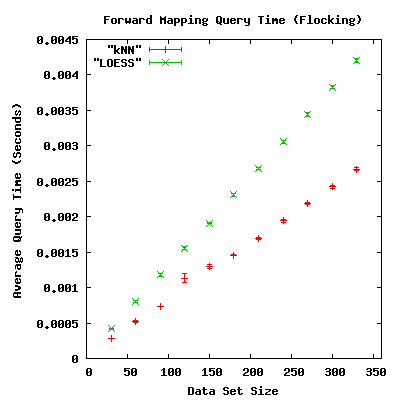
\includegraphics[scale=.4]{images/results_flocking/fmquery.png}
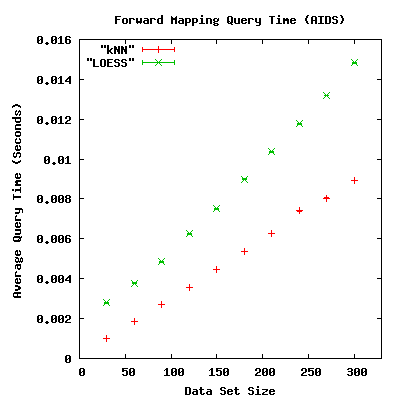
\includegraphics[scale=.4]{images/results_aids/aids-fmquery.png}
\caption{The average number of seconds required to query the Flocking (left) and AIDS (right) forward mappings.
The error bars show the 95\% confidence interval for the mean.}
\label{fig:fmquery}
\end{figure}



\begin{figure}[ht]
\centering
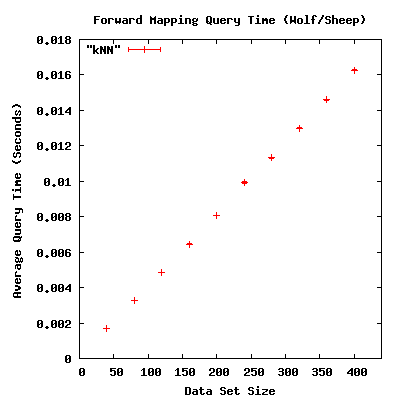
\includegraphics[scale=.5]{images/results_wolfsheep/fm-query.png}
\caption{The average number of seconds required to query the Wolf Sheep Predation forward mappings.
The error bars show the 95\% confidence interval for the mean.}
\label{fig:wolfsheepfmquery}
\end{figure}


\begin{table}[ht]
  \caption{Average Time for Individual Runs of ABMs}
  \centering
  \begin{tabular}{c c}
    \hline \hline
    ABM & Average Time Per Run (seconds)\\
    \hline
    Fires & 0.17\\
    Flocking & 8.20\\
    AIDS & 4.61\\
    Wolf Sheep Predation & 6.51\\
    \hline
  \end{tabular}
  \label{table:runtimes}
\end{table}


Online computation time is the average time required to query the forward mapping.
Since the forward mapping intends to replace the need for manual experimentation with ABMs, the forward mapping query should be significantly faster than actually running the ABM.
The average number of seconds required to query each of the ABMs in these experiments are listed in Table \ref{table:runtimes}.
As shown in Figure \ref{fig:fmquery} and Figure \ref{fig:wolfsheepfmquery}, the average query time is far below that of actually running the ABM.
For example, about two thousand Flocking forward mapping queries can be performed per Flocking ABM run.
Both LOESS and kNN have a linear rate of growth, which is as expected, because as more points are added to the training set, the more points that must be iterated over.
Naturally, problems with more system-level properties will require more time.

 \subsection{Reverse Mapping}

  \subsubsection{Accuracy vs. Forward Mapping}

The accuracy of the reverse mapping is measured as how well it approximates the forward mapping.
To measure this, for each simplex in the reverse mapping, the center point of the simplex has its system-level property values predicted with the forward mapping, and with the average the values at the corners.
The values at the knots have no error, since they were generated with the forward mapping.
Therefore, the points furthest away from these corners are most likely to have the greatest error.

\begin{figure}[ht]
\centering
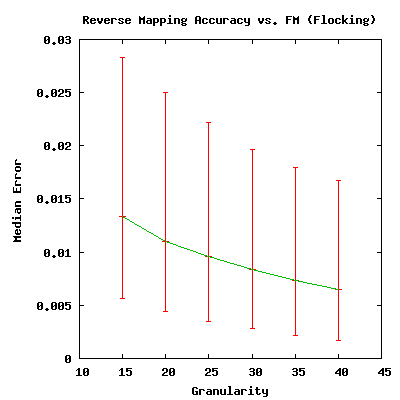
\includegraphics[scale=.5]{images/results_flocking/rmacc.png}
\caption{The median difference in the forward mapping and the reverse mapping in predictions for the Flocking domain.
The error bars show the upper and lower quartile of errors measured.}
\label{fig:flockrmacc}
\end{figure}

Results for the accuracy of the flocking domain are shown in Figure \ref{fig:flockrmacc}.
The median error of the reverse mapping with a granularity of 40 is about .007, which pales in comparison to the .05 error (see Figure \ref{fig:flockfmacc}) between the forward mapping and the actual ABM.
Therefore, the error incurred by the reverse mapping is relatively insignificant, especially when sometimes the error can cancel out the forward mapping error (i.e., the error from the reverse mapping and forward mapping is not additive).


\begin{figure}[ht]
\centering
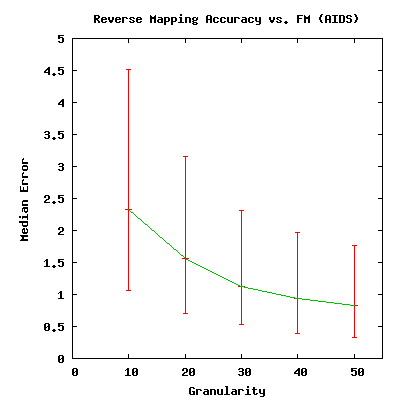
\includegraphics[scale=.5]{images/results_aids/aids-rmacc.png}
\caption{The median difference in the forward mapping and the reverse mapping in predictions for the AIDS domain.
The error bars show the upper and lower quartile of errors measured.}
\label{fig:aidsrmacc}
\end{figure}

Similar conclusions can be made about the accuracy of the reverse mapping for the AIDS domain, which are plotted in Figure \ref{fig:aidsrmacc}.
The median error for this domain with a granularity of 50 is below one person.
That is, in the most erroneous place in each simplex, the reverse mapping will predict the forward mapping's prediction within one person.
This error is about six times less than the error incurred by the forward mapping, for this domain.



  \subsubsection{Offline Computation Time}

\begin{figure}[ht]
\centering
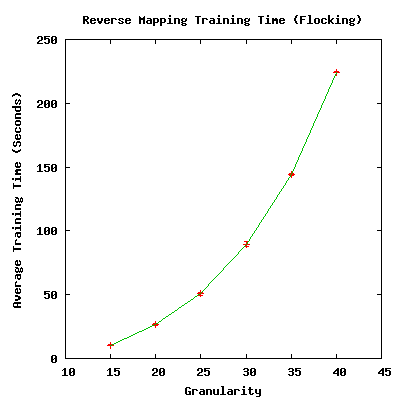
\includegraphics[scale=.5]{images/results_flocking/rmtraining.png}
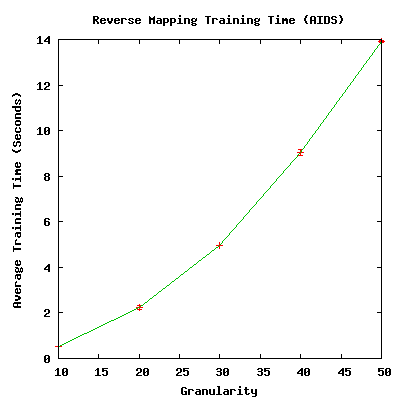
\includegraphics[scale=.5]{images/results_aids/aids-rmtraining.png}
\caption{The average number of seconds required to train the Flocking (left) and AIDS (right) reverse mappings.
The error bars show the 95\% confidence interval for the mean.}
\label{fig:farmtraining}
\end{figure}



The process of training the reverse mapping involves querying the forward mapping to generate the knots and then building the simplical complex from these knots.
Figure \ref{fig:farmtraining} shows the training time, based on granularity for the Flocking and AIDS domains.
At 40 granularity, the reverse mappings required approximately 9 seconds and 225 seconds to train for the AIDS domain and the Flocking domain, respectively.

For both the AIDS and Flocking domains, the required amount of time to train is acceptable, since it is computed offline.
However, there is a very large difference for the same granularity, given just one dimension difference in the configuration space (AIDS has two configuration parameters, while Flocking has three).
Unfortunately, the training time and memory is exponential in respect to the dimensionality.
Since each dimension is split granularity $g$ times, there are a total of $2 g^d$ simplexes, where $d$ is the dimensionality of the configuration space.
The coefficient of ``2" comes from the fact that each grid location is split into two simplexes.
Therefore, the memory required and the computation time required grow quickly with more dimensions.
The results from the Wolf Sheep Predation (with a configuration space dimensionality of five) are omitted because a granularity low enough to allow the experiments to run in a reasonable amount of time yielded poor accuracy.

Possible general methods for avoiding this computational problem are left as future work, which include optimization using the forward mapping and scaling granularity.
The simplest fix is to sample less configuration parameters at once and to learn individual reverse mappings for subsets of the configuration space.
Much information and qualitative information can still be gathered from these smaller mappings.


  \subsubsection{Online Computation Time}

\begin{figure}[ht]
\centering
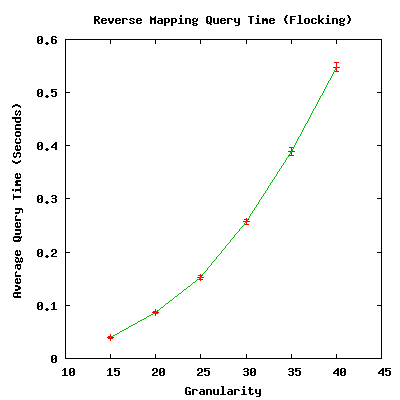
\includegraphics[scale=.5]{images/results_flocking/rmquery.png}
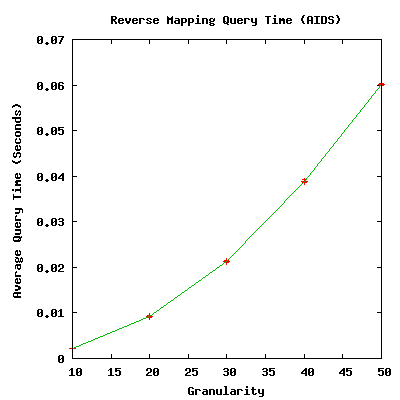
\includegraphics[scale=.5]{images/results_aids/aids-rmquery.png}
\caption{The average number of seconds required to query the Flocking (left) and AIDS (right) reverse mappings.
The error bars show the 95\% confidence interval for the mean.}
\label{fig:farmquery}
\end{figure}



Querying a reverse mapping requires the submapping for each system-level property to be searched for intersections.
Each simplex must be checked for intersections, so the running time of the query is based directly on the number of simplexes.
Since the number of simplexes grow at $O(g^d)$, the query is polynomial time, in respect to granularity.
This relationship is reflected in the results shown in Figure \ref{fig:farmquery}.
Similar to the training time, the query time for Flocking and AIDS are significantly different due to the additional configuration dimension in the Flocking domain.
In both these domains, queries were generally less than half a second, which is acceptable performance.



\section{Summary and Conclusions}

In summary, the forward mapping performed exceptionally well in comparison to the baselines provided.
The forward mapping is an accurate and quick tool for predicting real-valued system-level properties, as well as predicting the probability of a threshold effect (such as wolf extinction).
\fw was able to provide a general solution to this problem, proven by applying the same approaches to all four domains.

The reverse mapping solutions generated by \fw model the forward mapping accurately.
However, the computational and space complexity grow quickly with dimensionality, which make this approach intractable for highly-dimensional domains.
For the one-, two-, and three-dimensional configuration spaces presented in the results, granularities of forty produced accurate results within a reasonable about of time.



